\chapter{Ist Refactoring immer sinnvoll?}
\section{Beobachten statt vorhersagen}


\chapter{Sicherheit gewinnen, ohne den Code zu verstehen}
\section{Sicherheit durch Tests}
Die wohl einfachste Möglichkeit die Korrektheit von Software zu überprüfen, ist das Testen. In der Softwareentwicklung gibt es verschiedene Arten, wie richtiges Verhalten, einzelne Codeabschnitte oder ganze Produkte getestet werden können. Einige dieser Arten werden im folgenden aufgelistet.
\begin{itemize}
  \item \textbf{Unit Tests:} Testen von bla
  \item \textbf{Whiteboxtests:} Testen von bla
\end{itemize}
\section{Sicherheit durch Handwerkskunst}
\section{Sicherheit durch Werkzeuge}
\lipsum[1] % Dummy text

\begin{wrapfigure}{r}{0.4\textwidth}
  \centering
  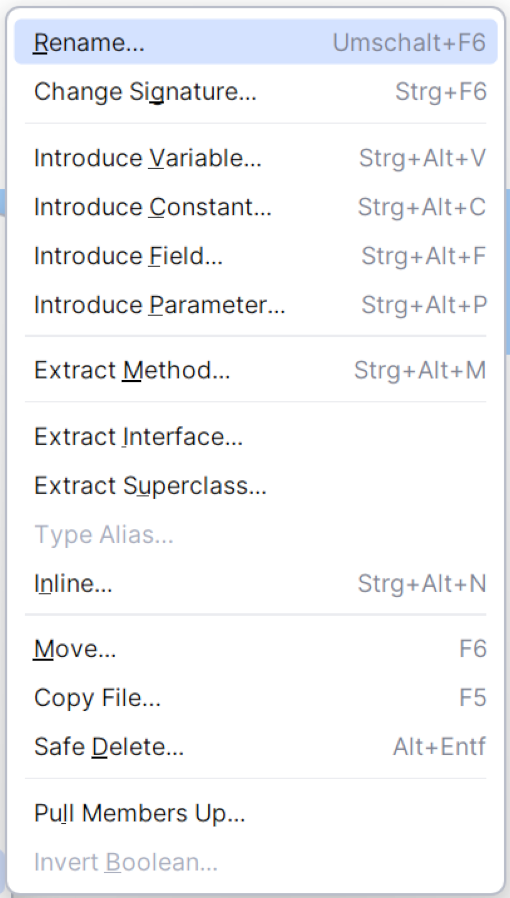
\includegraphics[width=0.35\textwidth]{Bilder/screenshotWebstorm} % Replace with your image file
  \caption{Screenshot WebStorm Refactoring-Tools \cite{webstorm.2024}}
\end{wrapfigure}

\lipsum[2-4] % More dummy text
\section{Sicherheit durch formale Verifikation}
\section{Sicherheit durch Fehlertoleranz}